\documentclass[main.tex]{subfiles}
\graphicspath{{./img}}

\begin{document}
    
\section{Proposed system}\label{sec-system}

This section is dedicated to designing the system that will be used to implement ITS in the
vehicle simulator software. A framework dedicated for generic MAS-based ITS system
implementation will be designed, utilizing the principles and paradigms gathered in the
preceding sections (\ref{its}, \ref{mas}). Firstly, the \emph{micro-architecture} will be
defined, i.e. the specification of the system's actors (agents) - their features,
characteristics, state variables and their goals, as well as interfaces to the environment.
This will form the elementary foundation that will be used to build an actual system. As a
follow up, agent interaction interface will be defined. This will for example include
knowledge sharing, conflict resolution and overall communication interface proposal, including
shared vocabulary and communication layers definition. The interaction interface will,
subsequently, lead to the \emph{macro-architecture} proposal. The structure of the system and
its behaviour will be defined. This will, among other topics, include discussing the
organizational and functional structure. The motivation behind functional structure definition
will be to define the behaviorist capabilities of the system and its configuration. The main
underlying motivation behind the organizational structure definition will be to facilitate the
aspect of control of the system. These steps should, in the end, lead to a full system
specification that will serve as a framework to implement agent-based ITSs in an interactive
vehicle simulator.

\subsection{Agent architecture}

As per the previous section(s), where the individual MAS architectures have been reviewed
(section \ref{mas}), it was decided to utilize  the \emph{hybrid \textsubscript{3}T
architecture\footnote{To remind the reader of the architecture's general structure, its
schematic is shown below (fig. \ref{3-arch2}).}} (section \ref{hybrid-arch}), which will offer
sufficient flexibility.  Such modeling flexibility is needed primarily because there won't be a
single, concrete system to model, but rather a generic system that will facilitate arbitrary
agent-based ITS implementation. As such, it makes sense to choose a hybrid architecture, which
will ensure there will be optimal balance between robust, reactive behaviour without giving up
capabilities to model complex behaviour.

Note that the architecture will be formally assume that the its implementation will be realized 
in an Object-Oriented Programming (OOP) paradigm. There are multiple reasons for that. Firstly, 
The nature of agent based systems, having their internal logic and interacting with the surroundings 
through pre-defined interface, corresponds to a large degree to the concepts of OOP, especially
the encapsulation mechanism.

%Nejak oduvodnit - the architecture will be proposed in such a way to be implemented by an 
% object-oriented programming approach

The individual layers/components will be outlined in the following section, in a bottom-up
fashion.

\begin{figure}[htbp]
    \centering
    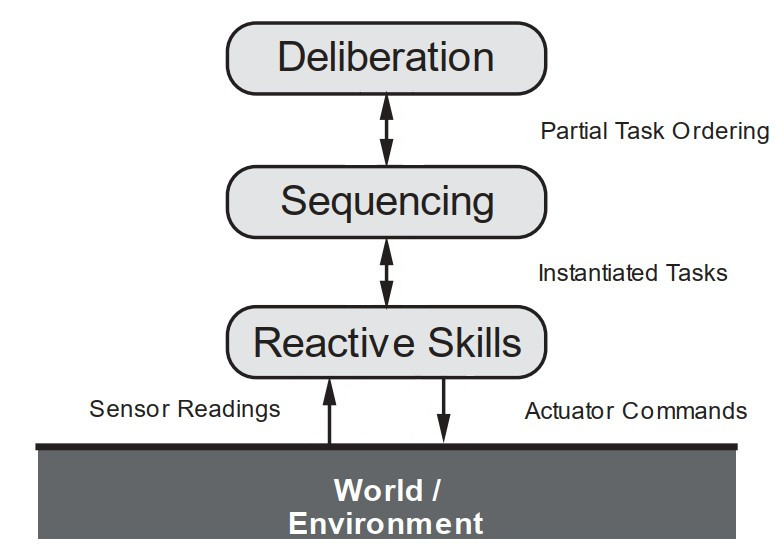
\includegraphics[width=.8\textwidth]{3t-arch.jpg}
    \caption{An architecture model of a \textsubscript{3}T hybrid architecture \cite{Bonasso1995}}
    \label{3-arch2}
\end{figure}

% The elementary characteristics that were defined according to \cite{ParasumannaGokulan2010}
% must shall also be taken into account: 

% \begin{itemize}
%     \item Situatedness
%     \item Autonomy 
%     \item Inferential capability 
%     \item Social behaviour 
% \end{itemize}

\subsubsection{The architecture layers}

In this section, the individual layers of the architecture will be defined. The layers' definition will 
adhere to the characteristics of the \textsubscript{3}T architecture. For each layer, it's purpose and 
relation to other layers will be described, together with technical implementation guidelines, such as 
configuration etc.

\textbf{Reactive skills layer \\\& Physical modules}

This layer encapsulates all the \emph{skills} the agent is able to do. These are the 
most primitive types of its behaviour\footnote{The original author of the architecture refers to them 
as Reactive Action Packages (RAPs) \cite{Firby1987}.}. For example, a skill might be to slow
down or to follow a vehicle in case of vehicle-based agent. Skills are usually activated one at a time, 
activated by the superior layers. This creates a level of abstraction, comparable to the principle found 
in Object Oriented Programming, where the superior unit (sequencer in this case) does not care how the 
given instruction will be executed. The sequencer only cares about the use-case and output of available
skills. 

In practice, each skill will be an individual script that will be synchronously, sequentially run. Inside 
the script, it will be possible to interact with the agent's interface, mainly its sensors or communication 
modules. The sensor and communication modules may provide an additional level of abstraction,
with exposed interface which will be defined by the architecture but configurable by the user.
This will mostly involve defining parameters of physical characteristics of the module, such 
as signal range, or error rate. Speaking of error rate, a skill will be also able to return a 
failure state to enable fail-safe behaviour. 

This essentially means that the skills will interact with another layer, which we could call the
\emph{Physical module layer}. This will be an elementary unit, which must be bound to a specific agent type. 
Therefore, the assigned modules will determine which skills the agent will be able to perform.  

\textbf{Sequencing layer}

The sequencing layer is responsible for queuing and execution of the individual skills. It is the 
intermediate layer between the reactive skill layer and deliberative planning layer. 

Apart from the trivial FIFO skills queuing, the sequencer will manage concurrent queues with different 
priorities, as the agent has to conform to a dynamic environment. Because indirect communication (i.e. 
broadcasting) will be featured in the proposed system, asynchronous skill sequencing will also be 
implemented using \emph{callbacks}. Usage of this feature can be simply argued by the fact that in traffic, 
the state of environment is changing rapidly, thus relying on sensory feedback would often not be enough 
to avoid faulty behaviour. Furthermore, there is a vast number of ITS solutions that utilize the 
broadcaster-subscriber principle, such as CACC systems and C-ITS systems in general.

\textbf{Deliberation layer}



\clearpage

\end{document}